\chapter{PHÂN TÍCH VÀ THIẾT KẾ HỆ THỐNG}

\section{Phân tích yêu cầu}
\subsection{Yêu cầu chức năng}
\begin{itemize}
    \item \textbf{Quản lý mật khẩu:} Thêm, sửa, xóa, xem các mục nhập mật khẩu.
    \item \textbf{Mã hóa/Giải mã:} Bảo vệ dữ liệu mật khẩu bằng mã hóa AES-256-GCM.
    \item \textbf{Tạo mật khẩu mạnh:} Tự động tạo mật khẩu ngẫu nhiên theo các tiêu chí (độ dài, ký tự đặc biệt, số...).
    \item \textbf{Quản lý danh mục:} Phân loại mật khẩu theo các danh mục (ví dụ: Công việc, Cá nhân, Ngân hàng).
    \item \textbf{Tìm kiếm:} Tìm kiếm nhanh các mục nhập mật khẩu.
    \item \textbf{Sao lưu và phục hồi:} Tự động sao lưu dữ liệu và cung cấp khả năng phục hồi từ các bản sao lưu.
    \item \textbf{Nhập/Xuất dữ liệu:} Hỗ trợ nhập/xuất dữ liệu từ/ra file JSON hoặc CSV.
    \item \textbf{Tự động khóa:} Tự động khóa ứng dụng sau một khoảng thời gian không hoạt động.
    \item \textbf{Tạo shortcut (Windows):} Tự động tạo shortcut trên desktop khi chạy lần đầu.
\end{itemize}

\subsection{Yêu cầu phi chức năng}
\begin{itemize}
    \item \textbf{Bảo mật:} Dữ liệu phải được bảo vệ chống lại truy cập trái phép và các cuộc tấn công.
    \item \textbf{Hiệu năng:} Ứng dụng phải hoạt động mượt mà, thời gian mã hóa/giải mã và tìm kiếm nhanh chóng.
    \item \textbf{Độ tin cậy:} Dữ liệu không được mất mát hoặc hỏng hóc. Hệ thống sao lưu phải hoạt động ổn định.
    \item \textbf{Khả năng sử dụng:} Giao diện phải trực quan, dễ hiểu và dễ thao tác.
    \item \textbf{Khả năng mở rộng:} Kiến trúc hệ thống nên cho phép dễ dàng thêm các tính năng mới.
\end{itemize}

\section{Thiết kế kiến trúc hệ thống}
AuraCrypt được thiết kế theo kiến trúc phân lớp, tách biệt rõ ràng các thành phần để dễ bảo trì và mở rộng.

\begin{figure}[H]
    \centering
    % TODO 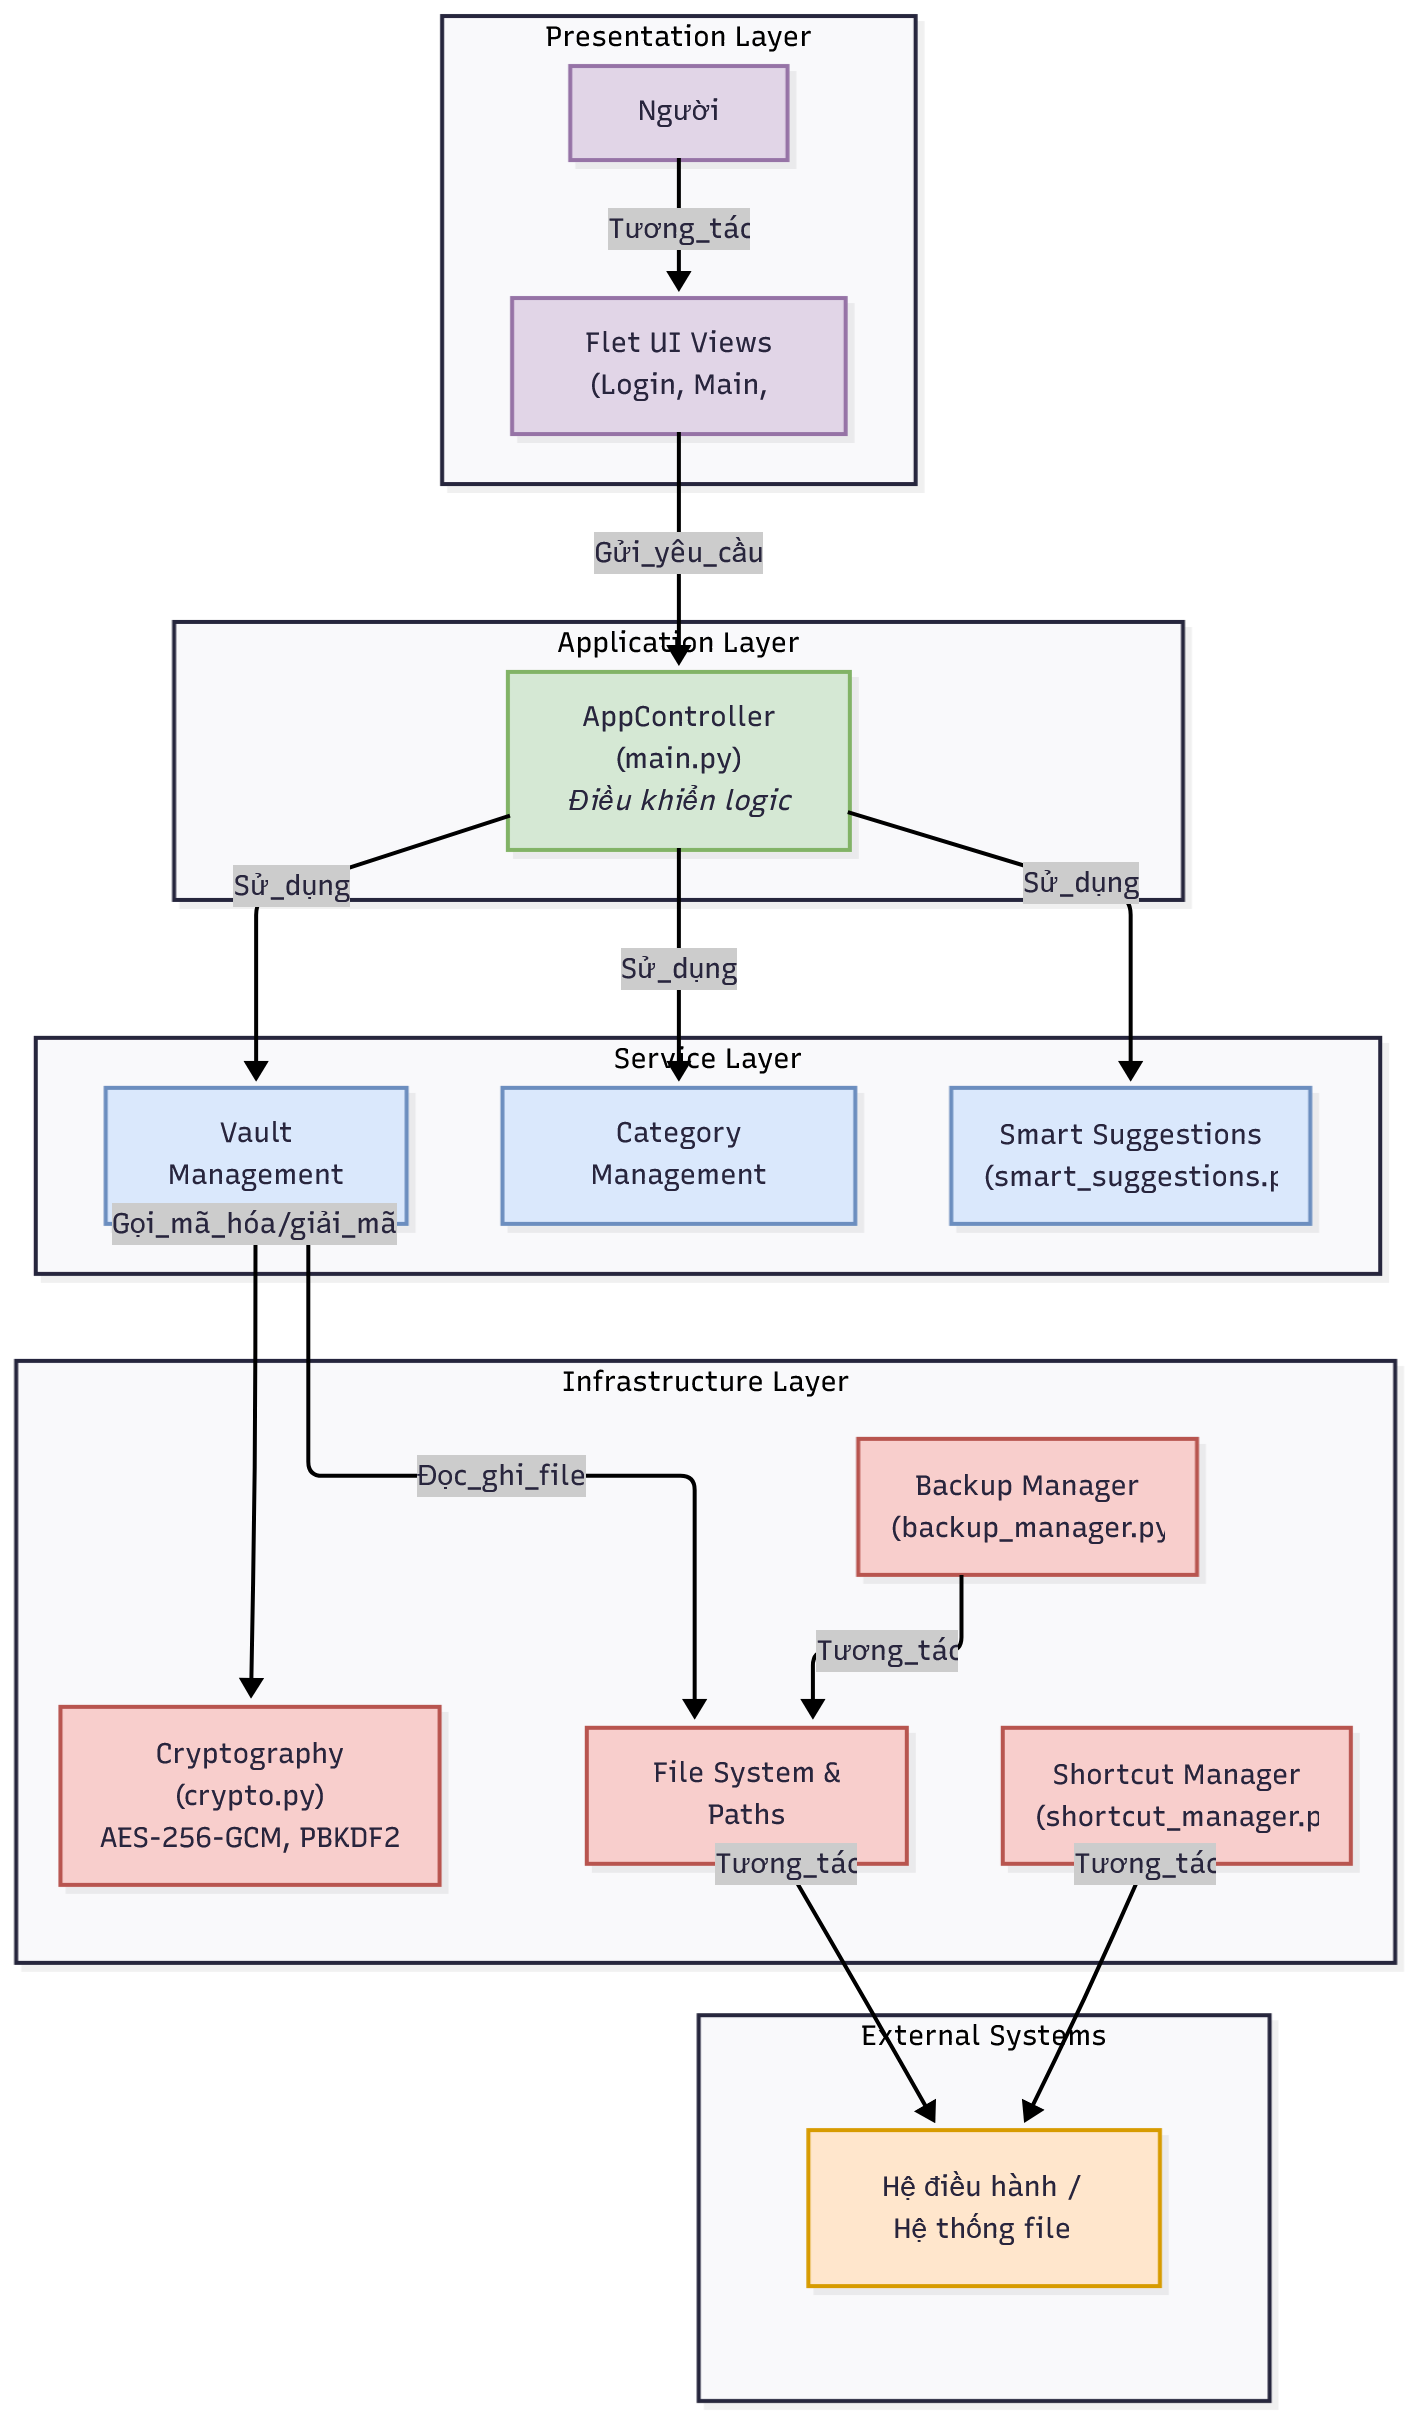
\includegraphics[width=0.8\textwidth]{images/architecture_diagram.png}
    \caption{Kiến trúc tổng quan của AuraCrypt}
    \label{fig:architecture_diagram}
\end{figure}
\textbf{Các lớp chính:}
\begin{itemize}
    \item \textbf{Presentation Layer (Lớp giao diện):} Xử lý các tương tác với người dùng thông qua Flet UI. Bao gồm các view (login, main vault, settings).
    \item \textbf{Application Layer (Lớp ứng dụng):} Chứa logic điều khiển chính của ứng dụng, tương tác với các lớp dưới để thực hiện các yêu cầu của người dùng.
    \item \textbf{Service Layer (Lớp dịch vụ):} Cung cấp các dịch vụ cốt lõi như quản lý vault, tạo mật khẩu, quản lý danh mục.
    \item \textbf{Infrastructure Layer (Lớp hạ tầng):} Bao gồm các module xử lý mã hóa, đọc/ghi file, sao lưu và các tương tác với hệ điều hành (ví dụ: tạo shortcut).
\end{itemize}

\section{Thiết kế cơ sở dữ liệu (Cấu trúc Vault)}
Dữ liệu mật khẩu được lưu trữ dưới dạng một file JSON đã mã hóa.
\begin{lstlisting}[caption=Cấu trúc dữ liệu vault mã hóa]
{
    "salt": "base64_encoded_salt",
    "nonce": "base64_encoded_nonce",
    "ciphertext": "base64_encoded_encrypted_data"
}
\end{lstlisting}
Trong đó, `ciphertext` chứa một đối tượng JSON đã mã hóa với cấu trúc sau:
\begin{lstlisting}[caption=Cấu trúc dữ liệu nội dung vault (chưa mã hóa)]
{
    "master_key_fingerprint": "hash_of_derived_key",
    "entries": [
        {
            "id": "uuid",
            "service": "Tên dịch vụ",
            "username": "Tên người dùng",
            "password": "Mật khẩu",
            "url": "URL liên quan",
            "category": "Danh mục",
            "notes": "Ghi chú",
            "created_at": "timestamp",
            "updated_at": "timestamp"
        }
    ],
    "categories": [
        "Danh mục 1",
        "Danh mục 2"
    ],
    "settings": {
        "auto_lock_timeout": 900,
        "clipboard_clear_delay": 15
    }
}
\end{lstlisting}
\subsection{Quản lý dữ liệu sao lưu}
Các bản sao lưu được lưu trong thư mục \texttt{backups} dưới dạng \texttt{vault\_YYYYMMDD\_HHMMSS.bak}.

\section{Thiết kế giao diện người dùng (UI/UX)}
Giao diện người dùng được thiết kế dựa trên nguyên tắc tối giản, hiện đại và dễ sử dụng.
\begin{itemize}
    \item \textbf{Màn hình Đăng nhập/Thiết lập:} Đơn giản, rõ ràng, hướng dẫn người dùng thiết lập mật khẩu chủ lần đầu.
    \item \textbf{Màn hình chính (Vault):} Hiển thị danh sách mật khẩu, thanh tìm kiếm, bộ lọc danh mục và các nút chức năng (thêm, sửa, xóa).
    \item \textbf{Form thêm/sửa mật khẩu:} Các trường nhập liệu rõ ràng, tích hợp nút tạo mật khẩu mạnh.
\end{itemize}

\begin{figure}[H]
    \centering
    % TODO 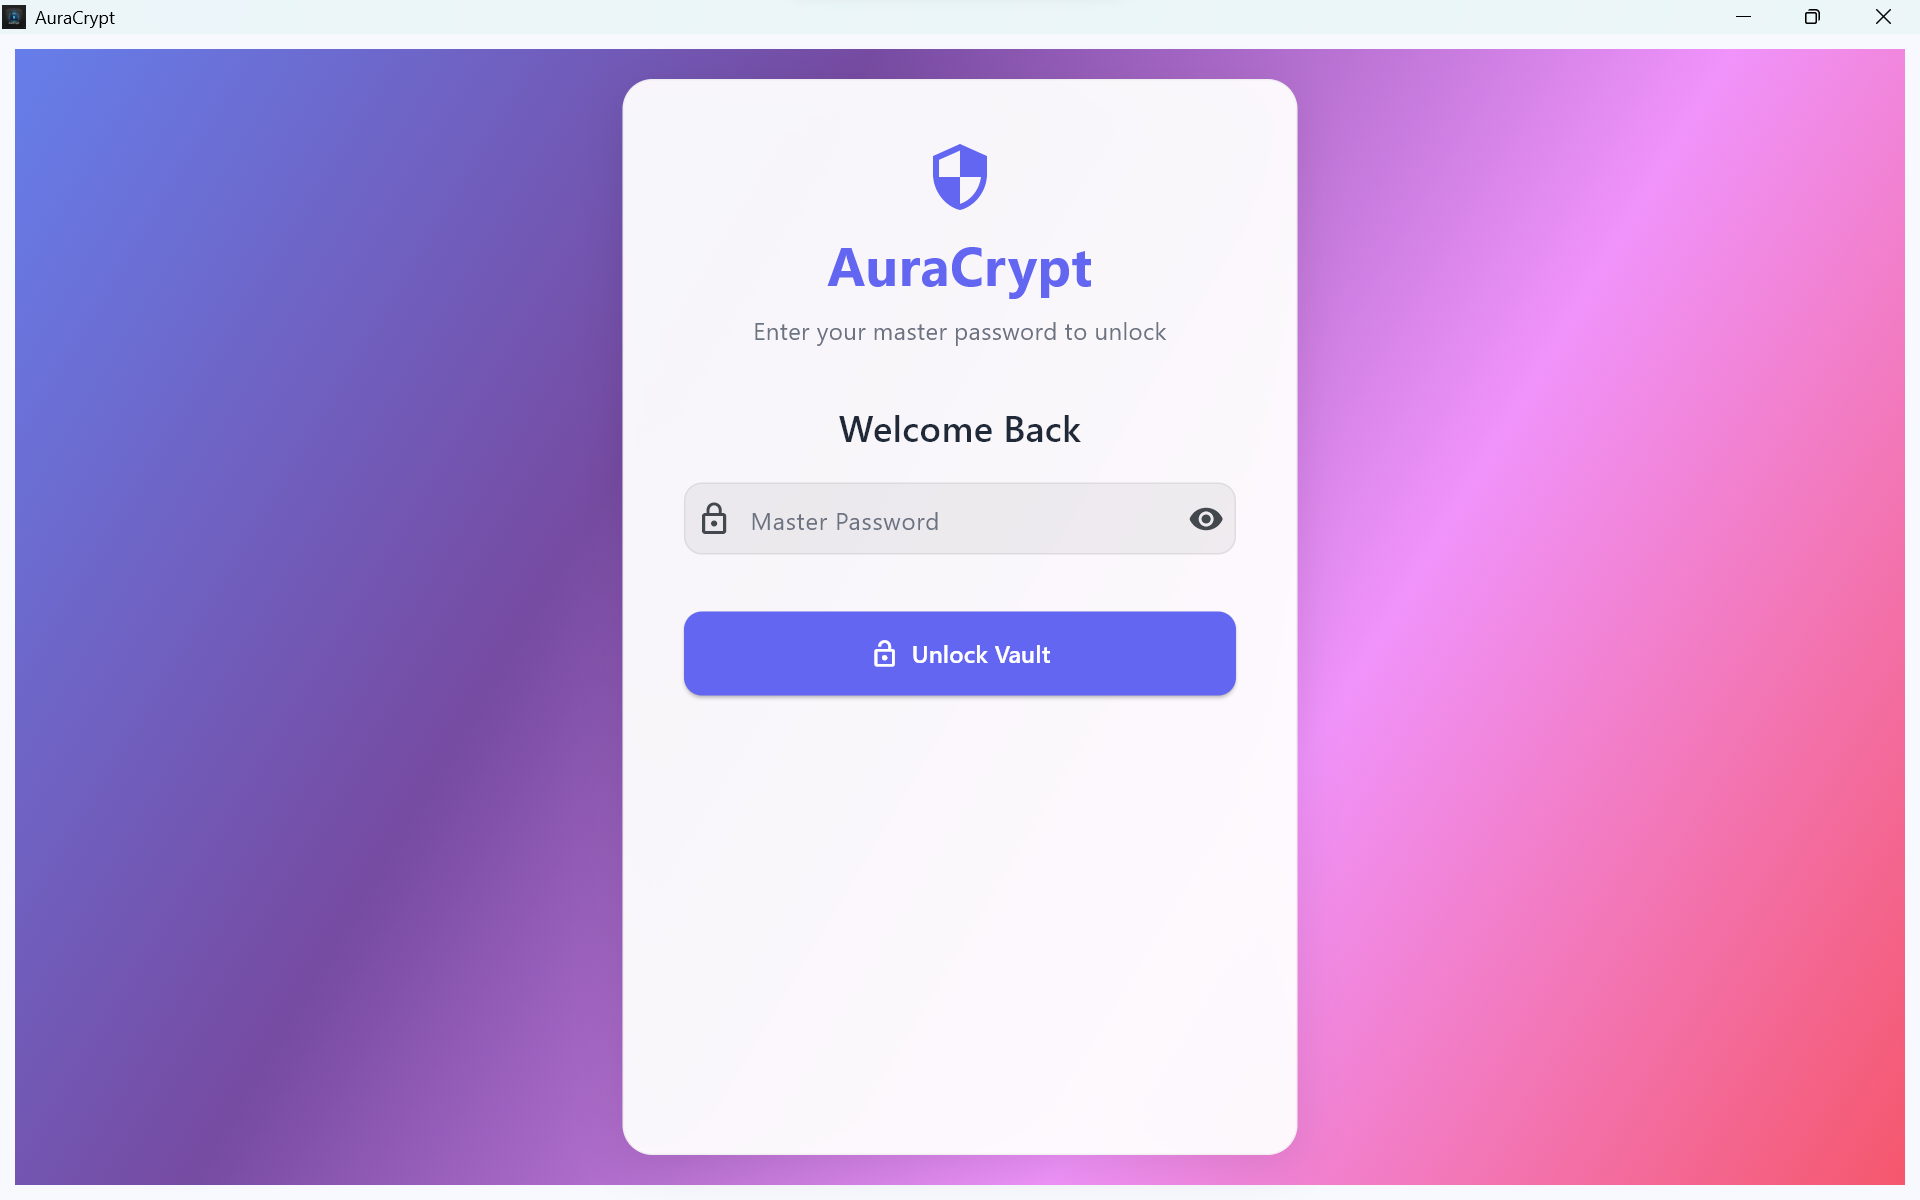
\includegraphics[width=0.7\textwidth]{images/mock_login_screen.png}
    \caption{Thiết kế giao diện màn hình Đăng nhập}
    \label{fig:login_screen}
\end{figure}

\begin{figure}[H]
    \centering
    % TODO 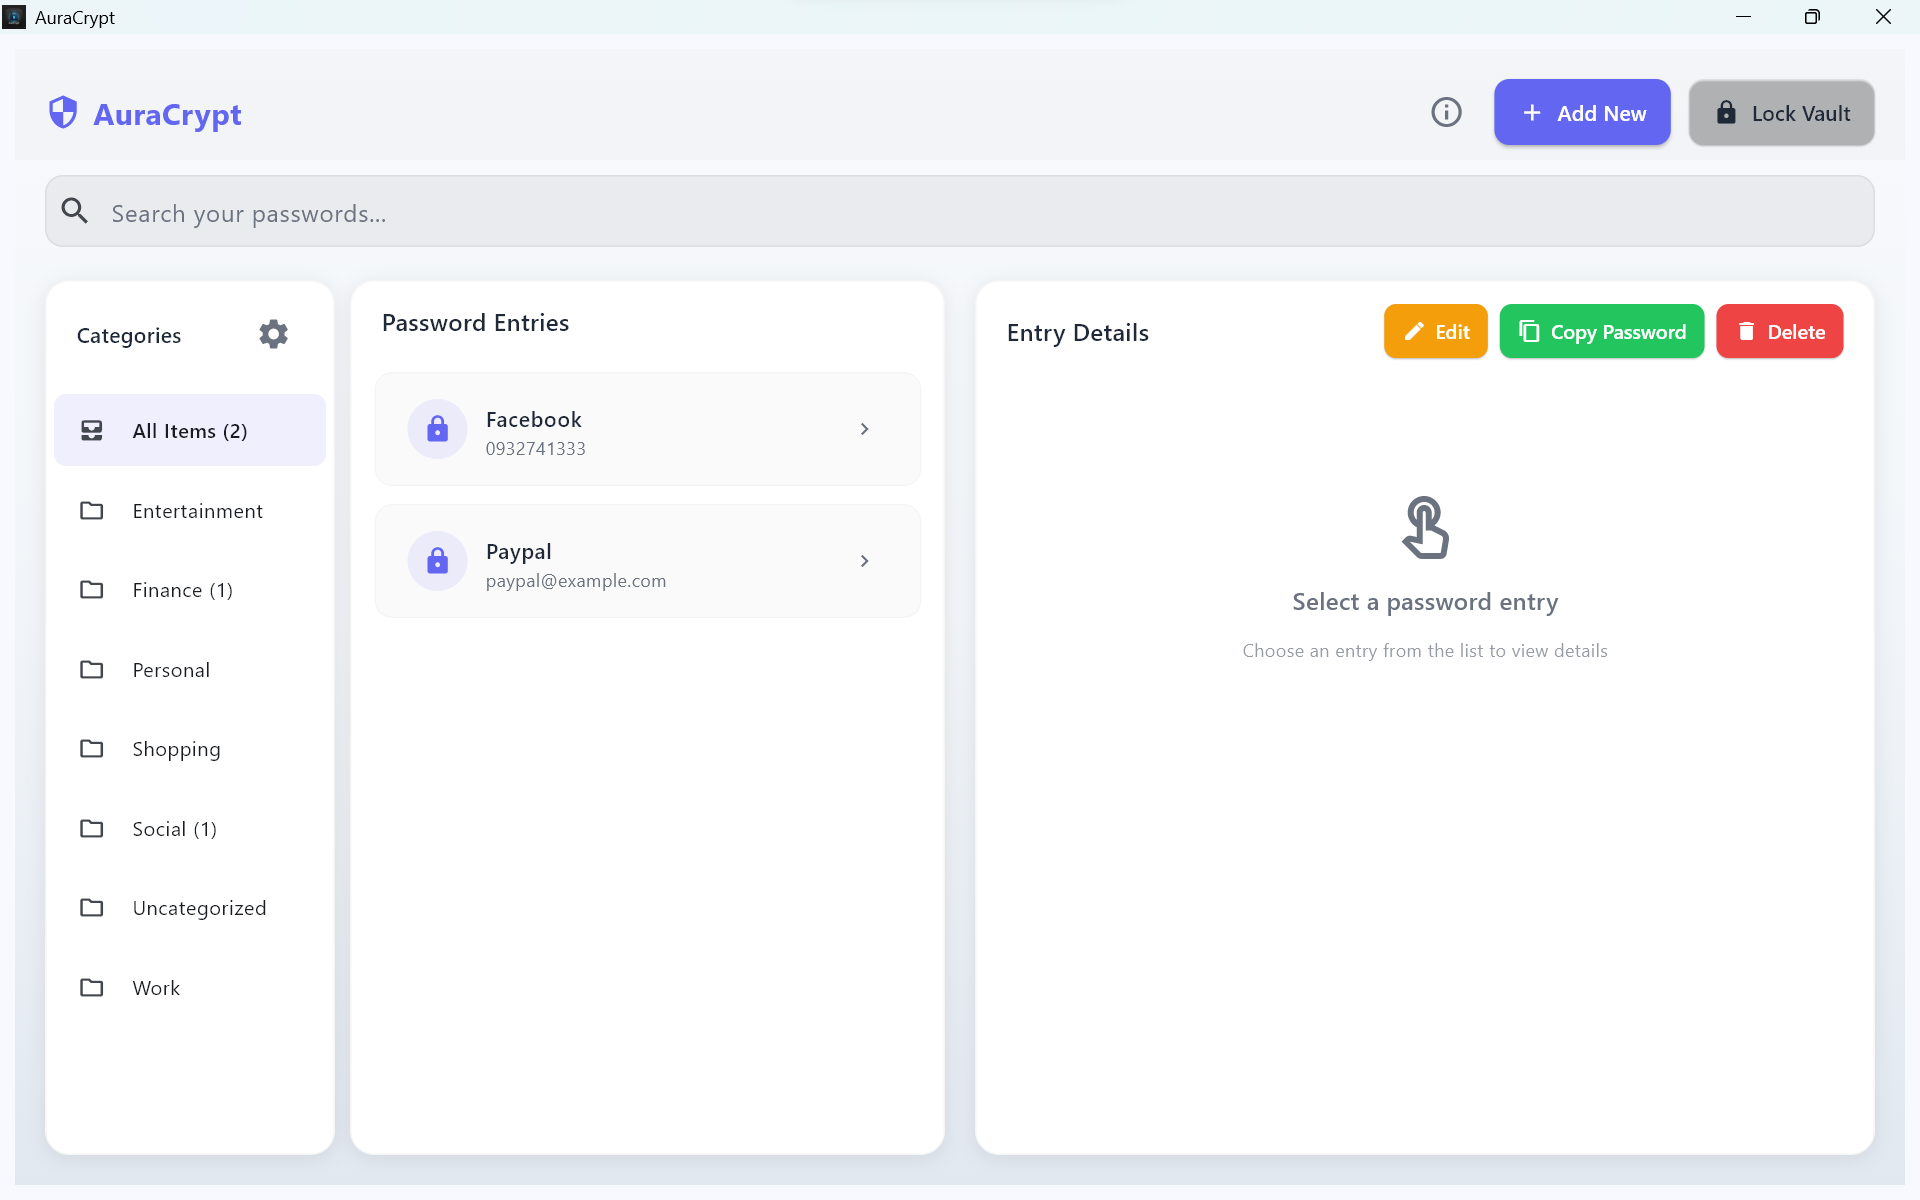
\includegraphics[width=0.7\textwidth]{images/mock_main_screen.png}
    \caption{Thiết kế giao diện màn hình chính}
    \label{fig:main_screen}
\end{figure}
\newpage